% ============================================================================
% Digital Finance for Supervision - A0 Conference Poster
% MSCA DIGITAL Network Workshop at the European Central Bank
% December 3, 2026
% ============================================================================
\documentclass[a0paper,portrait,25pt]{tikzposter}

% --- Packages ---
\usepackage[T1]{fontenc}
\usepackage[utf8]{inputenc}
\usepackage{helvet}
\renewcommand{\familydefault}{\sfdefault}
\usepackage{xcolor}
\usepackage{amssymb}
\usepackage{bm}
\usepackage{enumitem}
\usepackage{tabularx}
\usepackage{booktabs}
\usepackage{multicol}
\usepackage{qrcode}
\usepackage[hidelinks]{hyperref}
\usepackage{fontawesome5}
\usepackage{ragged2e}

% --- Colors ---
\definecolor{ecbblue}{HTML}{003399}
\definecolor{ecbgold}{HTML}{FFD700}
\definecolor{digitalblue}{HTML}{2E5090}
\definecolor{darkbg}{HTML}{1a1a2e}
\definecolor{lightbg}{HTML}{F0F0F0}
\definecolor{lightblue}{HTML}{E8EEF7}
\definecolor{lightgold}{HTML}{FFF8DC}
\definecolor{medgray}{HTML}{666666}

% --- tikzposter theme customization ---
\usetheme{Default}

\definecolorstyle{ECBStyle}{
  \definecolor{colorOne}{HTML}{003399}
  \definecolor{colorTwo}{HTML}{2E5090}
  \definecolor{colorThree}{HTML}{FFD700}
}{
  \colorlet{backgroundcolor}{white}
  \colorlet{framecolor}{ecbblue}
  \colorlet{titlefgcolor}{white}
  \colorlet{titlebgcolor}{ecbblue}
  \colorlet{blocktitlebgcolor}{ecbblue}
  \colorlet{blocktitlefgcolor}{white}
  \colorlet{blockbodybgcolor}{white}
  \colorlet{blockbodyfgcolor}{darkbg}
  \colorlet{innerblocktitlebgcolor}{digitalblue}
  \colorlet{innerblocktitlefgcolor}{white}
  \colorlet{innerblockbodybgcolor}{lightblue}
  \colorlet{innerblockbodyfgcolor}{darkbg}
}
\usecolorstyle{ECBStyle}

\defineblockstyle{ECBBlock}{
  titlewidthscale=1.0,
  bodywidthscale=1.0,
  titlecenter,
  titleoffsetx=0pt,
  titleoffsety=0pt,
  bodyoffsetx=0pt,
  bodyoffsety=0pt,
  bodyverticalshift=0pt,
  roundedcorners=12,
  linewidth=2pt,
  titleinnersep=10mm,
  bodyinnersep=12mm
}{
  \draw[color=framecolor, fill=blocktitlebgcolor, line width=\blocklinewidth,
        rounded corners=\blockroundedcorners]
    (blocktitle.south west) rectangle (blocktitle.north east);
  \draw[color=framecolor!30, fill=blockbodybgcolor, line width=\blocklinewidth*0.5,
        rounded corners=\blockroundedcorners]
    (blockbody.south west) rectangle (blockbody.north east);
}
\useblockstyle{ECBBlock}

% Title format
\definetitlestyle{ECBTitle}{
  width=\paperwidth,
  roundedcorners=0,
  linewidth=0pt,
  innersep=20mm,
  titletotopverticalspace=10mm,
  titletoblockverticalspace=25mm
}{
  \begin{scope}[line width=0pt]
    \draw[fill=ecbblue, draw=none]
      (\titleposleft, \titleposbottom) rectangle (\titleposright, \titlepostop);
    % Gold accent lines
    \draw[ecbgold, line width=4pt]
      (\titleposleft, \titleposbottom) -- (\titleposright, \titleposbottom);
    \draw[ecbgold, line width=2pt]
      (\titleposleft, \titleposbottom+8mm) -- (\titleposleft+300mm, \titleposbottom+8mm);
  \end{scope}
}
\usetitlestyle{ECBTitle}

% --- Title ---
\title{\bfseries Digital Finance for Supervision}
\author{MSCA DIGITAL Network Workshop at the European Central Bank}
\institute{Bringing Together ECB Supervision Experts and DIGITAL Network Researchers --- December 3, 2026}

% --- Document ---
\begin{document}

\maketitle

% Gold accent bar below title (manual)
\node[anchor=north, minimum width=\paperwidth, minimum height=6mm, fill=ecbgold, opacity=0.15]
  at ([yshift=-2mm]current page.north) {};

% ============================================================================
% ROW 1
% ============================================================================
\begin{columns}

% --- Column 1: Key Information ---
\column{0.33}

\block{Key Information}{
  \Large
  \begin{itemize}[leftmargin=18pt, itemsep=12pt, label={\color{ecbgold}\faIcon{chevron-right}}]
    \item \textbf{Date:} Thursday, December 3, 2026
    \item \textbf{Time:} 10:00\,--\,15:00 CET
    \item \textbf{Venue:} European Central Bank\\
          Sonnemannstrasse 20\\
          60314 Frankfurt am Main, Germany
    \item \textbf{Participants:} 30--50
    \item \textbf{Registration:} Free of charge
    \item \textbf{Format:} In-person workshop
    \item \textbf{Language:} English
    \item \textbf{Lunch:} Provided
  \end{itemize}

  \vspace{10mm}
  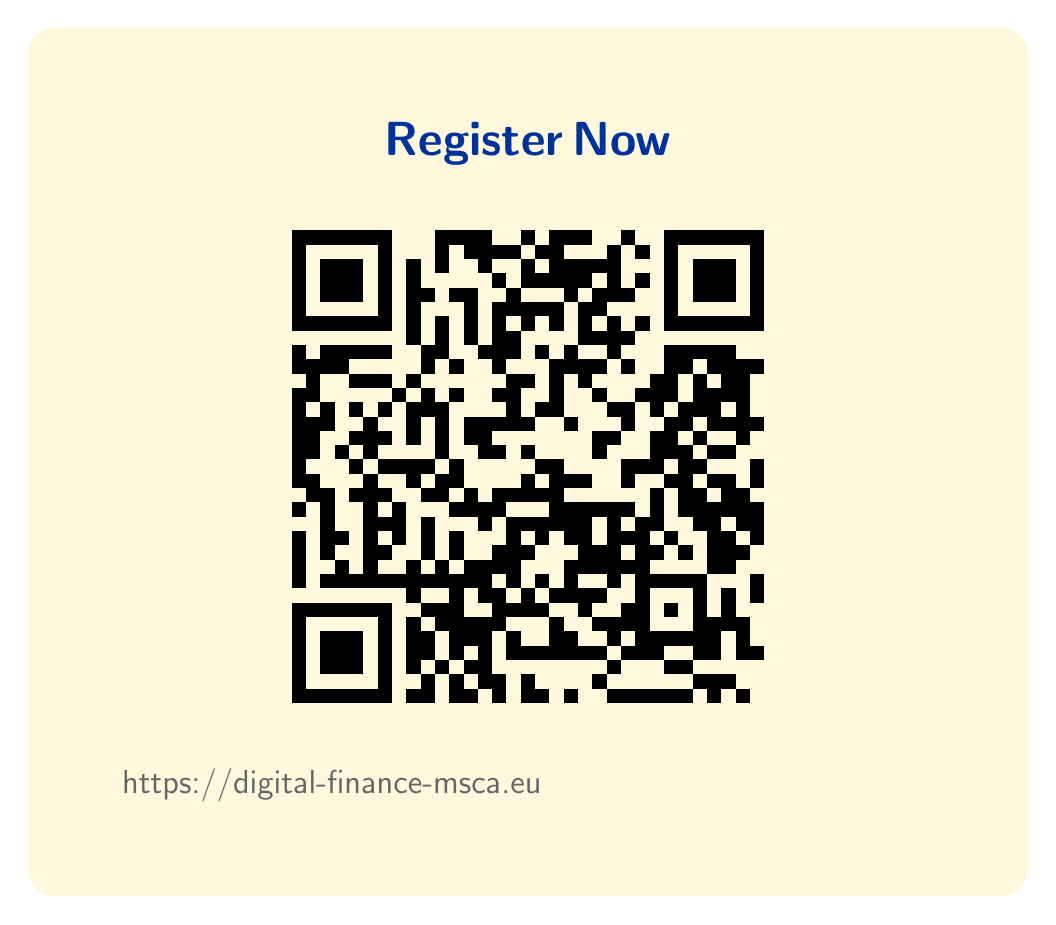
\begin{tikzpicture}
    \node[fill=lightgold, rounded corners=10pt, inner sep=12mm, text width=0.85\linewidth] {%
      \centering
      {\LARGE\bfseries\color{ecbblue} Register Now}\\[8mm]
      \qrcode[height=6cm]{https://digital-finance-msca.eu/events/ecb-workshop-2026}\\[8mm]
      {\large\color{medgray}\url{https://digital-finance-msca.eu}}
    };
  \end{tikzpicture}
}

% --- Column 2: Research Topics ---
\column{0.34}

\block{Research Topics}{
  % Topic 1
  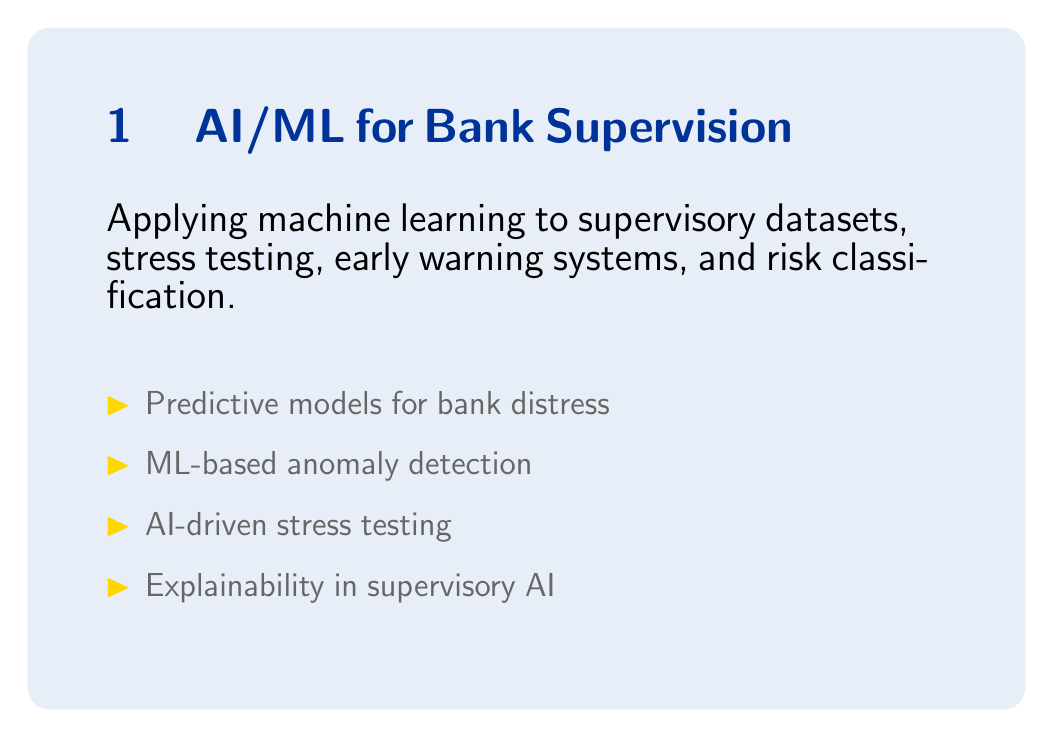
\begin{tikzpicture}
    \node[fill=lightblue, rounded corners=8pt, inner sep=10mm,
          text width=0.88\linewidth, align=left] {%
      {\LARGE\bfseries\color{ecbblue} 1 \quad AI/ML for Bank Supervision}\\[6mm]
      {\Large Applying machine learning to supervisory datasets, stress testing, early warning systems, and risk classification.}\\[5mm]
      {\large\color{medgray}
      \begin{itemize}[leftmargin=14pt, itemsep=4pt, label={\color{ecbgold}$\blacktriangleright$}]
        \item Predictive models for bank distress
        \item ML-based anomaly detection
        \item AI-driven stress testing
        \item Explainability in supervisory AI
      \end{itemize}}
    };
  \end{tikzpicture}

  \vspace{8mm}

  % Topic 2
  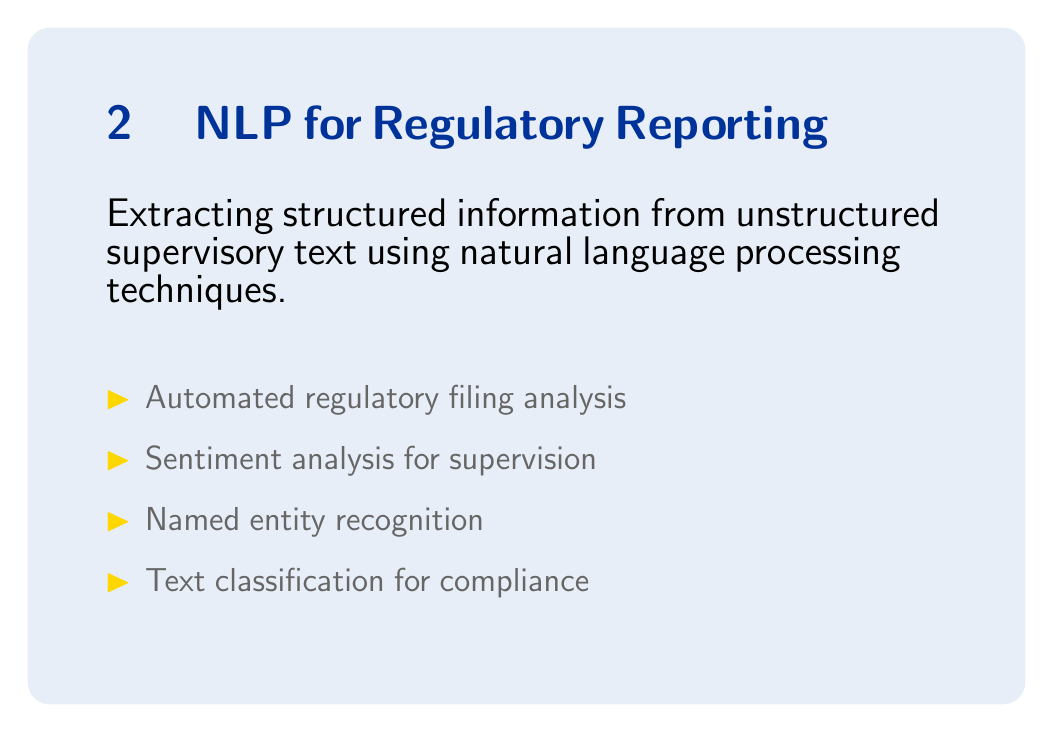
\begin{tikzpicture}
    \node[fill=lightblue, rounded corners=8pt, inner sep=10mm,
          text width=0.88\linewidth, align=left] {%
      {\LARGE\bfseries\color{ecbblue} 2 \quad NLP for Regulatory Reporting}\\[6mm]
      {\Large Extracting structured information from unstructured supervisory text using natural language processing techniques.}\\[5mm]
      {\large\color{medgray}
      \begin{itemize}[leftmargin=14pt, itemsep=4pt, label={\color{ecbgold}$\blacktriangleright$}]
        \item Automated regulatory filing analysis
        \item Sentiment analysis for supervision
        \item Named entity recognition
        \item Text classification for compliance
      \end{itemize}}
    };
  \end{tikzpicture}

  \vspace{8mm}

  % Topic 3
  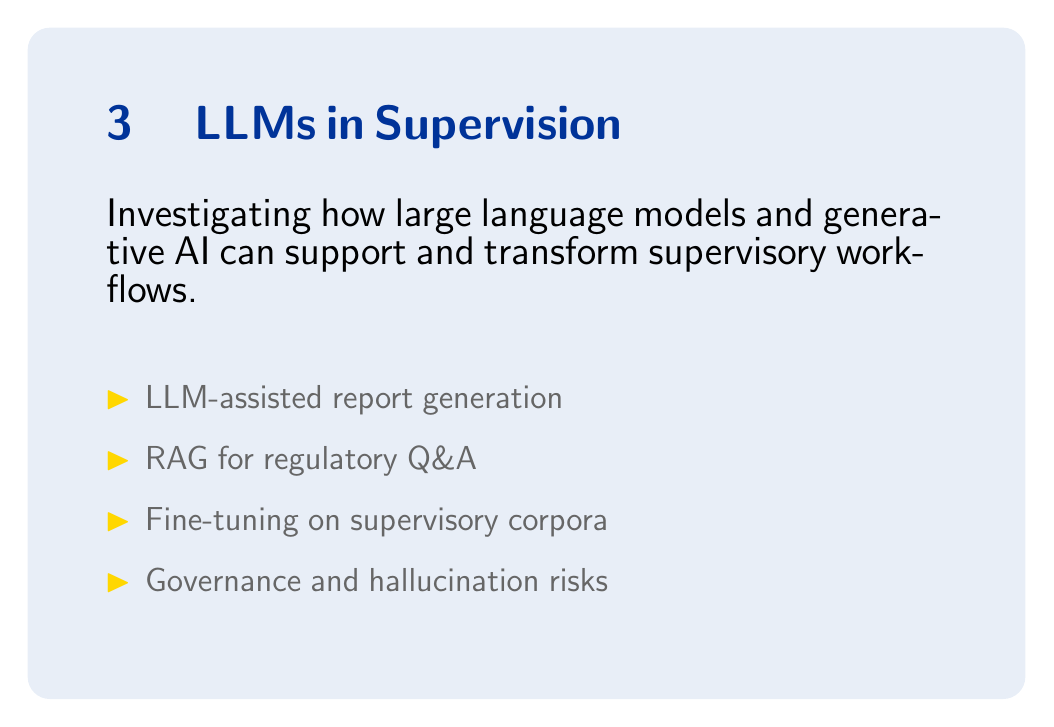
\begin{tikzpicture}
    \node[fill=lightblue, rounded corners=8pt, inner sep=10mm,
          text width=0.88\linewidth, align=left] {%
      {\LARGE\bfseries\color{ecbblue} 3 \quad LLMs in Supervision}\\[6mm]
      {\Large Investigating how large language models and generative AI can support and transform supervisory workflows.}\\[5mm]
      {\large\color{medgray}
      \begin{itemize}[leftmargin=14pt, itemsep=4pt, label={\color{ecbgold}$\blacktriangleright$}]
        \item LLM-assisted report generation
        \item RAG for regulatory Q\&A
        \item Fine-tuning on supervisory corpora
        \item Governance and hallucination risks
      \end{itemize}}
    };
  \end{tikzpicture}
}

% --- Column 3: Program Highlights ---
\column{0.33}

\block{Program Highlights}{
  \Large
  \renewcommand{\arraystretch}{1.5}
  \begin{tabularx}{\linewidth}{>{\bfseries\color{ecbblue}\large}l X}
    \multicolumn{2}{l}{\LARGE\bfseries\color{ecbblue} Morning}\\[3mm]
    10:00 & Registration \& Welcome Coffee\\
    10:15 & Opening Remarks\\
    10:30 & {\color{ecbgold}\textbf{Keynote Address 1}} (TBA)\\
    11:15 & Research Session 1:\\
           & AI/ML for Bank Supervision\\
           & {\normalsize\color{medgray}(3 research presentations)}\\[4mm]
    \multicolumn{2}{l}{\LARGE\bfseries\color{ecbblue} Lunch}\\[3mm]
    12:00 & {\color{medgray}Lunch Break \& Networking}\\[4mm]
    \multicolumn{2}{l}{\LARGE\bfseries\color{ecbblue} Afternoon}\\[3mm]
    13:00 & {\color{ecbgold}\textbf{Keynote 2 / Panel:}}\\
           & {\color{ecbgold}\textbf{LLMs in Supervision}} (TBA)\\
    13:45 & Research Session 2:\\
           & NLP \& SupTech Applications\\
           & {\normalsize\color{medgray}(3 research presentations)}\\
    14:30 & {\color{digitalblue}\textbf{Panel Discussion: The Future}}\\
           & {\color{digitalblue}\textbf{of Digital Supervision}}\\
    14:50 & Closing Remarks\\
  \end{tabularx}
  \renewcommand{\arraystretch}{1.0}

  \vspace{10mm}

  % Key numbers
  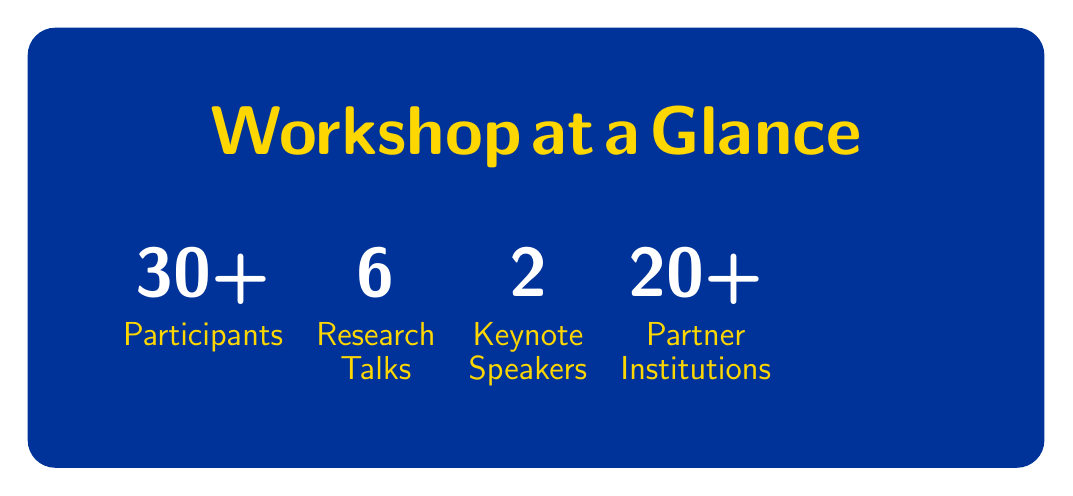
\begin{tikzpicture}
    \node[fill=ecbblue, rounded corners=10pt, inner sep=10mm, text width=0.9\linewidth] {%
      \centering
      {\Huge\bfseries\color{ecbgold} Workshop at a Glance}\\[10mm]
      \begin{tabular}{cccc}
        {\fontsize{48}{52}\selectfont\bfseries\color{white} 30+} &
        {\fontsize{48}{52}\selectfont\bfseries\color{white} 6} &
        {\fontsize{48}{52}\selectfont\bfseries\color{white} 2} &
        {\fontsize{48}{52}\selectfont\bfseries\color{white} 20+}\\[2mm]
        {\large\color{ecbgold} Participants} &
        {\large\color{ecbgold} Research} &
        {\large\color{ecbgold} Keynote} &
        {\large\color{ecbgold} Partner}\\
        & {\large\color{ecbgold} Talks} &
        {\large\color{ecbgold} Speakers} &
        {\large\color{ecbgold} Institutions}\\
      \end{tabular}
    };
  \end{tikzpicture}
}

\end{columns}

% ============================================================================
% ROW 2
% ============================================================================
\begin{columns}

% --- Column 1: Organizing Committee ---
\column{0.33}

\block{Organizing Committee}{
  {\LARGE\bfseries\color{ecbblue} Workshop Co-Chairs}

  \vspace{6mm}

  {\Large\bfseries Theodoros Mastrokostopoulos}\\
  {\large ECB Lead Organizer --- European Central Bank}

  \vspace{4mm}

  {\Large\bfseries Joerg Osterrieder}\\
  {\large DIGITAL Network Coordinator --- University of Twente}

  \vspace{10mm}
  {\color{ecbgold}\rule{0.6\linewidth}{2pt}}
  \vspace{6mm}

  {\LARGE\bfseries\color{ecbblue} Committee Members}

  \vspace{6mm}

  {\Large
  \begin{itemize}[leftmargin=14pt, itemsep=6pt, label={\color{ecbgold}\textbullet}]
    \item \textbf{Filippo Bartoli}\\{\large ECB Co-organizer, European Central Bank}
    \item \textbf{Daniel Pele}\\{\large Bucharest U. of Economic Studies}
    \item \textbf{Wolfgang H\"ardle}\\{\large HU Berlin / WU Vienna}
    \item \textbf{Maria Iannario}\\{\large University of Naples Federico II}
    \item \textbf{Codruta Mare}\\{\large Babes-Bolyai University}
    \item \textbf{Claudia Tarantola}\\{\large University of Milan}
    \item \textbf{Alessandra Tanda}\\{\large University of Pavia}
  \end{itemize}}
}

% --- Column 2: Partner Institutions ---
\column{0.34}

\block{Partner Institutions}{
  {\LARGE\bfseries\color{ecbblue} Beneficiary Partners}
  \vspace{4mm}

  {\Large
  \begin{multicols}{2}
  \begin{itemize}[leftmargin=14pt, itemsep=4pt, label={\color{digitalblue}\faIcon{university}}]
    \item University of Twente (NL)
    \item WU Vienna (AT)
    \item U. Naples Federico II (IT)
    \item Kaunas U. Technology (LT)
    \item Bucharest U. Econ. Studies (RO)
    \item Babes-Bolyai U. (RO)
    \item Cardo AI (IT)
    \item Poznan U. Economics (PL)
    \item U. Pavia (IT)
    \item U. Milan (IT)
    \item Bern U. Applied Sciences (CH)
  \end{itemize}
  \end{multicols}}

  \vspace{6mm}
  {\color{ecbgold}\rule{0.5\linewidth}{2pt}}
  \vspace{6mm}

  {\LARGE\bfseries\color{ecbblue} Associated Partners}
  \vspace{4mm}

  {\Large
  \begin{multicols}{2}
  \begin{itemize}[leftmargin=14pt, itemsep=4pt, label={\color{ecbgold}\faIcon{handshake}}]
    \item European Central Bank (DE)
    \item Deutsche Bank (DE)
    \item Raiffeisen Bank Int'l (AT)
    \item Swedbank (LT)
    \item Intesa Sanpaolo (IT)
    \item Deloitte (IT)
    \item Fraunhofer ITWM (DE)
    \item EIT Digital (BE)
    \item Athena Research Centre (GR)
    \item Royalton Partners (LU)
    \item Bank for Int'l Settlements (CH)
  \end{itemize}
  \end{multicols}}
}

% --- Column 3: Call for Papers & Funding ---
\column{0.33}

\block{Call for Participation}{
  \begin{tikzpicture}
    \node[fill=lightgold, rounded corners=10pt, inner sep=12mm,
          text width=0.88\linewidth, align=left] {%
      {\LARGE\bfseries\color{ecbblue} We Welcome Contributions On:}\\[8mm]
      {\Large
      \begin{itemize}[leftmargin=14pt, itemsep=6pt, label={\color{ecbgold}\faIcon{check-circle}}]
        \item AI and machine learning for banking supervision
        \item Natural language processing for regulatory reporting and compliance
        \item Large language models for supervisory processes
        \item SupTech tools and applications
        \item Digital innovation in financial oversight
      \end{itemize}}\\[8mm]
      {\Large\color{medgray} Interested researchers are invited to submit abstracts via the workshop website. Participation is free of charge.}
    };
  \end{tikzpicture}

  \vspace{10mm}

  % Funding acknowledgment
  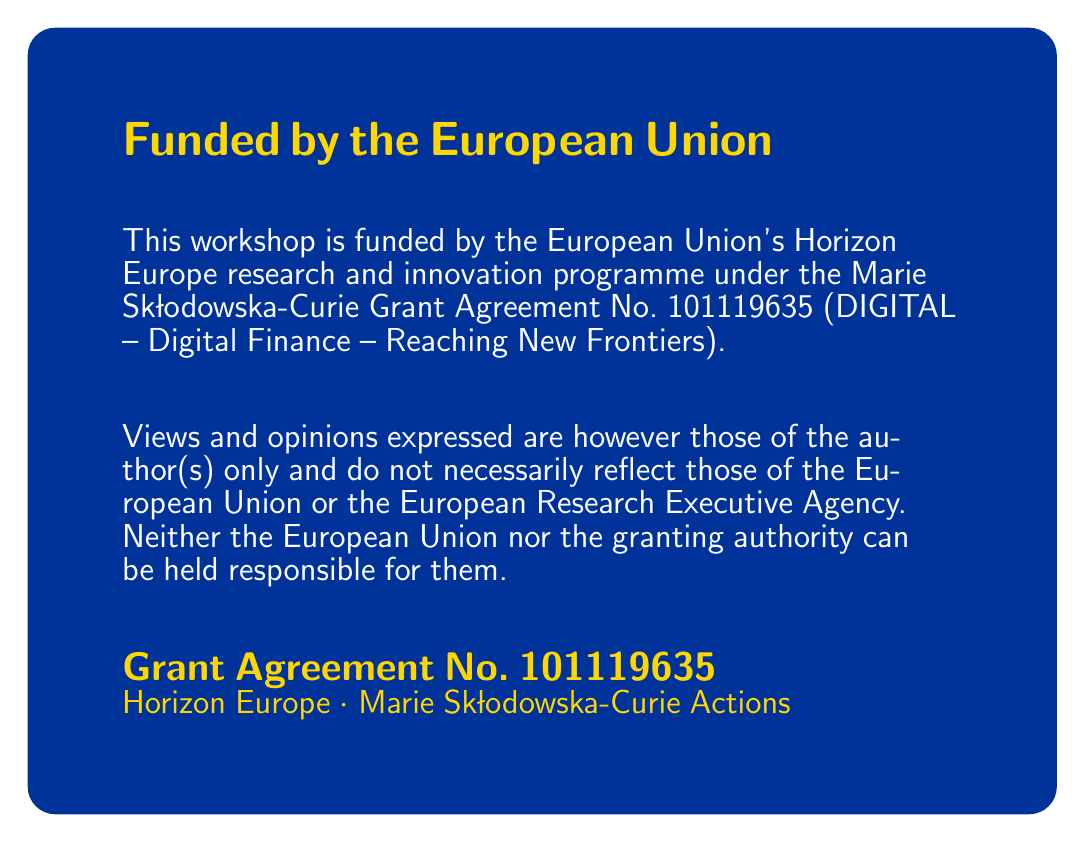
\begin{tikzpicture}
    \node[fill=ecbblue, rounded corners=10pt, inner sep=12mm,
          text width=0.88\linewidth, align=left] {%
      {\LARGE\bfseries\color{ecbgold} Funded by the European Union}\\[8mm]
      {\large\color{white}
      This workshop is funded by the European Union's Horizon Europe research and innovation programme under the Marie Sk\l{}odowska-Curie Grant Agreement No.\ 101119635 (DIGITAL -- Digital Finance -- Reaching New Frontiers).}\\[8mm]
      {\large\color{white!70}
      Views and opinions expressed are however those of the author(s) only and do not necessarily reflect those of the European Union or the European Research Executive Agency. Neither the European Union nor the granting authority can be held responsible for them.}\\[8mm]
      {\Large\bfseries\color{ecbgold} Grant Agreement No.\ 101119635}\\
      {\large\color{ecbgold} Horizon Europe $\cdot$ Marie Sk\l{}odowska-Curie Actions}
    };
  \end{tikzpicture}
}

\end{columns}

% ============================================================================
% BOTTOM BAR
% ============================================================================
\node[anchor=south, minimum width=\paperwidth, minimum height=35mm,
      fill=ecbblue, inner sep=10mm] at (current page.south) {%
  \begin{minipage}{0.95\paperwidth}
    \centering
    {\color{ecbgold}\rule{0.5\paperwidth}{1.5pt}}\\[6mm]
    {\fontsize{30}{34}\selectfont\color{white}\bfseries
      digital-finance-msca.eu
      \qquad\color{ecbgold}$\bm{\cdot}$\qquad
      \color{white} December 3, 2026
      \qquad\color{ecbgold}$\bm{\cdot}$\qquad
      \color{white} European Central Bank, Frankfurt}\\[4mm]
    {\large\color{ecbgold}
      DIGITAL -- Digital Finance -- Reaching New Frontiers
      $\cdot$ GA 101119635
      $\cdot$ Horizon Europe
      $\cdot$ MSCA}
  \end{minipage}
};

\end{document}
